%%%%%%%%%%%%%%%%%%%%%%%%%%%%%%%%%%%%%%%%%%%%%%%%%%%%%%%%%%%%%%%%%%%%%%%%%%%%%
% 26/05/2010
% edited by Bill Lampos
%
% Feel free to use (copy) the structure (latex formatting source code)
% but not the content of this document.
%
%%%%%%%%%%%%%%%%%%%%%%%%%%%%%%%%%%%%%%%%%%%%%%%%%%%%%%%%%%%%%%%%%%%%%%%%%%%%%
\documentclass[compress,red]{beamer}
%\documentclass{beamer}
\mode<presentation>

\usetheme{Warsaw}
%\usetheme{CambridgeUS}
%\usetheme{AnnArbor}
% other themes: Warsaw, AnnArbor, Antibes, Bergen, Berkeley, Berlin, Boadilla, boxes, CambridgeUS, Copenhagen, Darmstadt, default, Dresden, Frankfurt, Goettingen,
% Hannover, Ilmenau, JuanLesPins, Luebeck, Madrid, Maloe, Marburg, Montpellier, PaloAlto, Pittsburg, Rochester, Singapore, Szeged, classic

%\usecolortheme{beaver}
% color themes: albatross, beaver, beetle, crane, default, dolphin, dov, fly, lily, orchid, rose, seagull, seahorse, sidebartab, structure, whale, wolverine

\usefonttheme{serif}
% font themes: default, professionalfonts, serif, structurebold, structureitalicserif, structuresmallcapsserif

% pdf is displayed in full screen mode automatically
%\hypersetup{pdfpagemode=FullScreen}

% define your own colours:
\definecolor{Red}{rgb}{1,0,0}
\definecolor{Blue}{rgb}{0,0,1}
\definecolor{Green}{rgb}{0,1,0}
\definecolor{magenta}{rgb}{1,0,.6}
\definecolor{lightblue}{rgb}{0,.5,1}
\definecolor{lightpurple}{rgb}{.6,.4,1}
\definecolor{gold}{rgb}{.6,.5,0}
\definecolor{orange}{rgb}{1,0.4,0}
\definecolor{hotpink}{rgb}{1,0,0.5}
\definecolor{newcolor2}{rgb}{.5,.3,.5}
\definecolor{newcolor}{rgb}{0,.3,1}
\definecolor{newcolor3}{rgb}{1,0,.35}
\definecolor{darkgreen1}{rgb}{0, .35, 0}
\definecolor{darkgreen}{rgb}{0, .6, 0}
\definecolor{darkred}{rgb}{.75,0,0}

\xdefinecolor{olive}{cmyk}{0.64,0,0.95,0.4}
\xdefinecolor{purpleish}{cmyk}{0.75,0.75,0,0}

% \usepackage{beamerinnertheme_______}
% inner themes include circles, default, inmargin, rectangles, rounded

%\usepackage{beamerouterthemesmoothbars}
% outer themes include default, infolines, miniframes, shadow, sidebar, smoothbars, smoothtree, split, tree

%\useoutertheme{infolines}
\useoutertheme[subsection=false]{smoothbars}
\defbeamertemplate*{footline}{shadow theme}
{%
  \leavevmode%
  \hbox{\begin{beamercolorbox}[wd=.5\paperwidth,ht=2.5ex,dp=1.125ex,leftskip=.3cm plus1fil,rightskip=.3cm]{author in head/foot}%
    \usebeamerfont{author in head/foot}\insertframenumber\,/\,\inserttotalframenumber\hfill\insertshortauthor\,\,(\insertshortinstitute)
  \end{beamercolorbox}%
  \begin{beamercolorbox}[wd=.5\paperwidth,ht=2.5ex,dp=1.125ex,leftskip=.3cm,rightskip=.3cm plus1fil]{title in head/foot}%
    \usebeamerfont{title in head/foot}\insertshorttitle%
  \end{beamercolorbox}}%
  \vskip0pt%
}

% to have the same footer on all slides
%\setbeamertemplate{footline}[text line]{xxx xxx xxx}
%\setbeamertemplate{footline}[text line]{} % or empty footer

% include packages
\usepackage[all,knot]{xy}
\usepackage[symbol]{footmisc}
\usepackage{amsmath}
\usepackage{amssymb}
\usepackage{graphicx}
\usepackage{multicol}
\usepackage{multimedia}
\usepackage{setspace}
\usepackage{url}
\usepackage{xr}
\xyoption{arc}
\usepackage{appendixnumberbeamer}
\usepackage{biblatex}
\bibliography{references}

\title[Forecasting a Moving Target]{Forecasting a Moving Target: 
    Ensemble Models for ILI Case Count Predictions}
\author[Prithwish Chakraborty]{\scriptsize Prithwish Chakraborty$^{1,2}$, Pejman Khadivi$^{1,2}$,
  Bryan Lewis$^{3}$, \\
  Aravindan Mahendiran$^{1,2}$, Jiangzhuo Chen$^{3}$,  Patrick Butler$^{1,2}$,\\
  Elaine O. Nsoesie$^{3,4, 5}$, Sumiko R. Mekaru$^{4, 5}$, John S. Brownstein$^{4, 5}$,\\
Madhav V. Marathe$^{3}$, Naren Ramakrishnan$^{1,2}$}

\institute[prithwi@vt.edu]{\tiny ${}^1$Dept. of Computer Science, Virginia Tech, USA\\
${}^2$Discovery Analytics Center, Virginia Tech, USA\\
${}^3$NDSSL, Virginia Bioinformatics Institute, USA\\
${}^4$Children's Hopsital Informatics Program, Boston Children's Hopsital, USA\\
${}^5$Dept. of Pediatrics, Harvard Medical School, USA.}
{\color{red}\date{April 24, 2014}}

\begin{document}

\frame{
	\titlepage
}

\section[Outline]{}
\frame{\tableofcontents}

\section{Introduction}
\subsection{Problem Overview}
\frame{\frametitle{Problem Overview}
  \pause
  \begin{itemize}
    \item Predicting weekly Influenza-like-illness (ILI) case counts for
      15 Latin American countries
    \item Investigating different open source data-streams as possible surrogate 
      indicators of ILI 
  \end{itemize}
}

\subsection{Motivation}
\frame{\frametitle{Motivation}
  \begin{itemize}
    \item Traditional methods are often not enough!!
      \begin{itemize}
        \item ILI surveillance is not real-time - often lags several weeks
        \item Estimates are ``unstable'' - often revised over several months
      \end{itemize}
      \pause
    \item Can surrogate information be used to provide more stable and real time 
      estimates?
      \begin{itemize}
        \item Either ``non-physical indicators'' or ``physical indicators'' investigated
        \item How to handle the instability associated with ILI surveillance
      \end{itemize}. 
  \end{itemize}
}

%\iffalse
%\frame{\frametitle{Problem Overview}
  %{\onslide<2-> \begin{columns}
      %\column{0.5\textwidth}
      %abc
      %\column{0.5\textwidth}
      %def
    %\end{columns}
  %}
  %{\onslide<3-> \begin{columns}
      %\column{0.5\textwidth}
      %abc1
      %\column{0.5\textwidth}
      %def1
    %\end{columns}
  %}
%}
%\frame{\frametitle{Check}
  %\begin{columns}
    %\column{0.5\textwidth}
    %\begin{itemize}
      %\item<2-> a
      %\item<3-> b
      %\item<4-> c
    %\end{itemize}
    %\column{0.5\textwidth}
    %\begin{itemize}
      %\item<2-> a1
      %\item<3-> b1
      %\item<4-> c1
    %\end{itemize}
  %\end{columns}
%}
%\fi


\subsection{Key Contributions}
\frame{\frametitle{Key Contributions}
\begin{enumerate}
  \item Real-time prospective study - most studies till now have been 
    retrospective
    \pause
  \item Integrates both social and physical indicators 
    \pause
  \item Data level fusion vs Model level fusion?
    \pause
  \item Accounting for uncertainties in the official surveillance estimates
    \pause
  \item Investigate importance of different sources - Ablation test
\end{enumerate}
}

\section{Methods}
\frame{\frametitle{ Overall Framework}
  \begin{center}
  \includegraphics[height=0.7\textheight]{figures/ili_data_pipeline.pdf}
  \end{center}
  %Our ILI data pipeline, depicting 
%six different data sources used in this paper to forecast ILI case counts.

}

\subsection{Data Sources}
\frame{\frametitle{Data Sources}
\begin{itemize}
  \item Non-physical indicators
    \pause
    \begin{enumerate}
      \item Google Flu Trends - uses unpublished set of keywords
        \pause
      \item Custom User Keywords
        \begin{enumerate}
          \item Google Search Trends
          \item Healthmap News Feed
          \item Twitter Feed
        \end{enumerate}
    \end{enumerate}
    \pause
  \item Physical indicators
  \item Misc. Indicators
    \begin{enumerate}
      \item Opentable reservations
    \end{enumerate}
\end{itemize}
}

\frame{\frametitle{Google Flu Trends}
  \begin{center}
  \includegraphics[height=0.7\textheight]{figures/gft_vs_gst}
  \end{center}
}

\subsection{Custom User Keywords}
\frame{\frametitle{Finding Custom user keyword dictionary}
  A multiple step process :
  \begin{itemize}
    \item Started with a seed set of keywords from experts.
      \begin{itemize}
        \item Seed set contains words in Spanish, Portuguese, and English.
        \item example : \textit{gripe} (flu in Spanish)
      \end{itemize}
      \pause
    \item Pseudo-query expansion
      \begin{itemize}
        \item Crawled top 20 web-sites for each seed word.
        \item Crawled ``expert'' web-sites e.g. CDC.
        \item Crawled few other hand-picked sites.
        \item Top 500 frequently occurring words selected.
      \end{itemize}
      \pause
    \item Time series correlation analysis
      \begin{itemize}
        \item Used Google Correlate to find words with search history correlated 
          with ILI incidence curve.
        \item Interesting words such as \textit{ginger} and \textit{Acemuk} 
          found.
      \end{itemize}
      \pause
    \item Final filtering : {\color{blue}114} words
  \end{itemize}
}

\frame{\frametitle{\small GFT vs other non-physical indicators using custom keyword set}
  \begin{columns}
    \column{0.30\textwidth}
    \centering
    \includegraphics[width=1.05\textwidth, height=0.6\textheight]{figures/gst}
    \column{0.30\textwidth}
    \centering
    \includegraphics[width=1.05\textwidth, height=0.6\textheight]{figures/hm}
    \column{0.30\textwidth}
    \centering
    \includegraphics[width=1.05\textwidth, height=0.6\textheight]{figures/twitter}
  \end{columns}

  \begin{columns}
    \column{0.30\textwidth}
    \centering
    Google Search Trends (GST)
    \column{0.30\textwidth}
    \centering
    Healthmap
    \column{0.30\textwidth}
    \centering
    Twitter
  \end{columns}
}


\frame{\frametitle{Physical Indicators}
  \begin{columns}
    \column{0.5\textwidth}
    \begin{itemize}
      \item Meteorological data for every lat-long, worldwide, every 8 hours
      \item Humidity, Temperature, Rainfall
      \item Analyzing grid cells covering PAHO sites.
    \end{itemize}

    \column{0.5\textwidth}
  \begin{center}
  \includegraphics[scale=0.5]{figures/met}
  \end{center}

  \end{columns}
}


\frame{\frametitle{System framework once again!!}
  \begin{center}
  \includegraphics[height=0.7\textheight]{figures/ili_data_pipeline.pdf}
  \end{center}
}

\subsection{Matrix Factorization using Nearest Neighborhood}
\frame{\frametitle{Preliminaries}
  \begin{itemize}
    \item To find predictive model$f$
      \begin{equation*}
        \label{eq:problem}
        f: \mathcal{P}_t = f\left(\mathcal{P}, \mathcal{X}\right)
        \vspace{-1em}
      \end{equation*}
    \item Variable Setup
      \begin{equation*}
        \label{eq:regressionvector}
        \begin{array}{lcl}
          V_t & \equiv & \langle P_{t-\beta - \alpha}, \mathcal{X}_{t-\beta - \alpha}, P_{t + 1 -\beta-\alpha}, \mathcal{X}_{t + 1 - \beta-\alpha}, \dots, \\
              &        & P_{t-\alpha},\mathcal{X}_{t-\alpha} \rangle \\
          L_t & \equiv & P_{t}\\
        \end{array}
      \end{equation*}
    \item Parameters
      \begin{itemize}
        \item $\alpha$ : the {\it lookahead window length}
        \item $\beta$ :  the {\it lookback window length}
      \end{itemize}
  \end{itemize}
}
\frame{\frametitle{Matrix Factorization (MF)}
  \begin{itemize}
    \item Can find latent factors in the dataset.
      \pause

    \item Model
      \begin{equation*}
        \begin{array}{l}
         \widehat{\mathcal{M}}_{i,j} = b_{u,i} + U^T_i  F_j \\
         b_{i,j} = \bar{\mathcal{M}} + b_j 
        \end{array}
      \end{equation*}

    \pause
    \item Fitting
      \begin{equation}
        \begin{array}{l}
        \label{eq:matrix:fit}
        b_*, F, U   =  \textrm{argmin} (\sum \limits_{i=1}^{m-1} \left(\mathcal{M}_{i,n}  - \widehat{\mathcal{M}}_{i,n} \right)^2 \\ 
        \quad + \lambda_1(\sum \limits_{j=1}^{n}b_j^2 + \sum \limits_{i=1}^{m-1} || U_i||^2 + \sum \limits_{j=1}^{n} || F_j||^2))
      \end{array}
      \end{equation}
    \end{itemize}
}

\frame{\frametitle{Nearest Neighbor model (NN)}
  \begin{itemize}
    \item Impose non-linearity.
      \pause
    \item 

    $\mathcal{N}(i) = \lbrace k : \mbox{$V_k$ is one of the top  K nearest neighbors of $V_{i}$} \rbrace$ 

    \pause
    \item Fitting
      \begin{equation} \label{eq:nearestneighbor:pred}
        \begin{array}{l}
          \widehat{P}_{T'}  =  ({\sum\limits_{k \in \mathcal{N}(T')}
        \theta_{k}L_{k,T - \alpha}})
          /{\sum\limits_{k=1}^{K} \theta_{k}}\\
        \end{array}
      \end{equation}
  \end{itemize}
}

\frame{\frametitle{Matrix Factorization using Nearest Neighborhood (MFN)}
  \small
  \begin{itemize}
    \item Inspired from Koren et al.'s work$^*$ in Recommender systems.
      \pause
    \item 
      \begin{equation}
        \label{eq:model:matrixfactornbr}
        \begin{array}{l}
          \widehat{\mathcal{M}}_{i,j}  =   b_{i,j} + U_i^T F_j \\
                        \quad             + F_j |\mathcal{N}(i)|^{-\frac{1}{2}}\sum_{k \in N(i)} (\mathcal{M}_{i,k} - b_{i,k}) x_k \\
        \end{array}
      \end{equation}

    \pause
    \item Fitting
    \begin{equation}
      \label{eq:matrixnbr:fit}
      \begin{array}{l}
        b_*, F, U, x_*  = \textrm{argmin} (\sum \limits_{i=1}^{m-1} \left(\mathcal{M}_{i,n} - \widehat{\mathcal{M}}_{i,n}   \right)^2 \\
                    \,   + \lambda_2(\sum \limits_{j=1}^{n}b_j^2 +
                    \sum \limits_{i=1}^{m-1} || U_i||^2 + \sum
                    \limits_{j=1}^{n} || F_j||^2 + \sum \limits_k ||x_k||^2))
      \end{array}
      \end{equation}

  \end{itemize}
  \vspace{1em}
  {\scriptsize
  $^{*}$~\fullcite{koren2008factor}
}
}

\frame{\frametitle{Accuracy comparison}
  \begin{itemize}
    \item Quality Metric
      \begin{equation} 
          \label{eq:def:accuracy} 
          \mathcal{A} = \frac{4}{N_p}\sum \limits_{t=t_s}^{t_e}\left( 1 - \frac{|P_t -\hat{P}_t| }{max(P_t, \hat{P}_t, 10)}\right)
          \vspace{-0.5em}
      \end{equation} 
  \end{itemize}
}
\frame{\frametitle{Accuracy comparison}
  \begin{left}
    \includegraphics[width=\textwidth]{figures/table1}
  \end{left}
  {\onslide<2->
    \begin{itemize}
        \small
      \item On average, MFN has better performance over MF and NN
      \item In Mexico, MF has the best accuracy - possibly because the 2013 ILI season in Mexico
        was late by a few weeks than in usual.
    \end{itemize}
  }
}

\subsection{Model level vs Data level fusion}
\frame{\frametitle{Model level fusion}
  \begin{itemize}
    \item Output from models combined based on historical accuracy.
      \vspace{1em}
      \pause
    \item Model
      \begin{equation}
        \label{eq:fusion:predictionmatrix}
        {}_C\mathcal{M}_{t} = \left[\begin{array}{llll}
            {}_1\widehat{P}_{t}& \dots & {}_C\widehat{P}_t & P_t 
          \end{array}
        \right]
      \end{equation}

    \vspace{1em}
    \pause
    \item Fitting
      \begin{equation}
          \label{eq:fusion:matrixfactornbr}
          \begin{array}{l}
            {}_C \widehat{\mathcal{M}}_{i,j} =  \mu_i + {}_C b_{j} + {}_C U_i^T  {}_C F_j \\
            \, + {}_C F_j  |{}_C \mathcal{N}(i)|^{-\frac{1}{2}}
            \sum_{k \in {}_C N(i)} ({}_C\mathcal{M}_{i,k} - \mu_i + {}_C b_{k}) {}_Cx_k \\
          \end{array}
      \end{equation}
  \end{itemize}

}
\frame{\frametitle{Data level fusion}
  \begin{itemize}
    \item Feature vector is a tuple over all data set features.
     \[\mathcal{X}_t = \langle \mathcal{T}_t, \mathcal{W}_t \rangle\]
    \item Use MFN to fit the value
  \end{itemize}

}

\frame{\frametitle{Accuracy comparison}
  \begin{left}
    \includegraphics[width=\textwidth]{figures/table2}
  \end{left}
  {\onslide<2->
    \begin{itemize}
        \small
      \item On average, model level fusion produces better accuracy than data level fusion.
      \item Interesting deviations like Chile and El Salvador indicates that a possible 
        strategy could be a mix of data level and model fusion - however complexity of 
        training will increase manifold.
    \end{itemize}
  }
}

\section{Instability Analysis}
\frame{\frametitle{Uncertainty in official estimates}
  \begin{itemize}
    \item Can take up to several months to stabilize.
\begin{columns}
  
  \column{0.45\textwidth}
  \centering
    \includegraphics[width=0.95\textwidth]{figures/ArgentinaColombia.pdf}
  \column{0.45\textwidth}
  \centering
    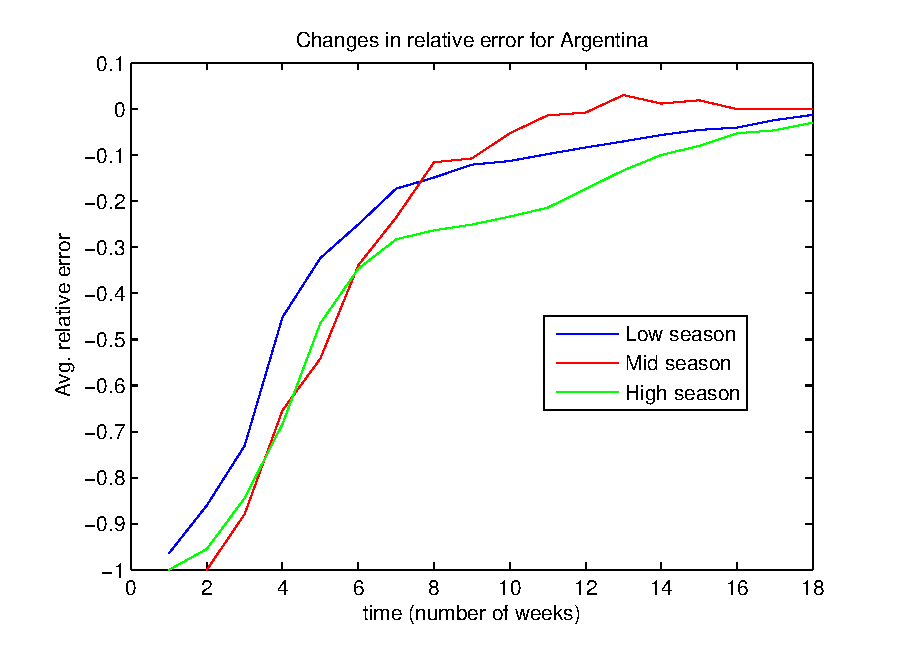
\includegraphics[width=0.95\textwidth]{figures/forpaper_seasonalAVGrelativeALLs_Argentina}
    \vspace{1em}
\end{columns}
  \item  Average relative error of PAHO count values with respect to stable values.
  (a) Comparison between Argentina and Colombia (b) Comparison between different 
  seasons for Argentina.
  \end{itemize}
}

\frame{\frametitle{Correcting uncertainty}
  \small
  \begin{itemize}
    \item Recognize high, low and mid-season months for countries.
    \item Variable setup
        \begin{small}
      \begin{equation*}
      \mathcal{P}_A{^S} = \left \{ (1,P_i^{(1)},\dot{P}_i,N_i^{(1)}),...,(m,P_i^{(m)},\dot{P}_i,N_i^{(m)}), ...  \right \}
      \end{equation*}
      \end{small}
      \vspace{-1em} 
    \item Correction Model
      \begin{equation}
      \hat{\dot{P}}_i^{(m)} = a_0 + a_1  m + a_2  P_i^{(m)} + a_3  N_i^{(m)}
      \label{eq:correctionpaho}
      \end{equation}
  \end{itemize}

  \pause
  \begin{left}
    \includegraphics[width=1.0\textwidth]{figures/table3}
  \end{left}
}

\section{Ablation Test}
\frame{\frametitle{Investigating importance of each source : Ablation Test}
  \begin{left}
      \includegraphics[width=1.0\textwidth]{figures/table4}
  \end{left}

  \pause
  \begin{itemize}
      \small
    \item Greater drop in accuracy $\implies$ Source more important
    \item Physical indicators are in general more important
    \item Still there is value in supplementing physical indicators with non-physical 
      indicators.
  \end{itemize}
}

\frame{\frametitle{Final look at real time predictions}
  \begin{columns}
    \column{0.35\textwidth}
    \scriptsize
      \begin{itemize}
        \item Weekly predictions sent out for 15 Latin American countries
        \item Predictions publicly available at 
          \url{http://embers.cs.vt.edu/embers/alerts/visualizer_isi}
      \end{itemize}
    \column{0.55\textwidth}
  \begin{center}
      \includegraphics[width=1.0\textwidth, height=0.3\textheight]{figures/at} \\
      \vspace{1em}
      \includegraphics[width=1.0\textwidth, height=0.3\textheight]{figures/at_2}
  \end{center}
  \end{columns}

}

\section{Conclusion}
\subsection{Extending to other sources: Opentable}
\frame{\frametitle{Conclusion: \\How to extend to other sources}
  \begin{itemize}
    \item Data about number of unreserved tables at restaurants in Mexico
  \end{itemize}
      \vspace{1em}
      \begin{center}
      \includegraphics[scale=0.65]{figures/table5}
      \end{center}
}

\subsection{Summary}
\frame{\frametitle{Summary}
  \begin{itemize}
    \item MFN performs better than MF, NN on average over individual sources 
      for predicting ILI case counts.
    \item In average there is a small advantage in combining models over different 
      sources than to combine data.
    \item Employing information about number of samples used and how far from the actual
      date the estimate is being updated by the reporting agency, we have been able to
      improve our overall accuracy by a quality score of 0.05.
    \item Generally physical indicators offer more advantage over non-physical indicators.
      However for some situations Healthmap and Twitter feed have been found to outperform 
      physical indicators.
    \item Experiments with Opentable reservation data shows that there is some 
      perceptible signal embedded w.r.t to ILI case counts.
  \end{itemize}
}

\frame{\frametitle{Future Work}
  \begin{itemize}
    \item Reconcile these phenomenological models with true epidemiological models.
    \item Explore inter-country characteristics of ILI profiles.
  \end{itemize}
}

\frame{\frametitle{Acknowledgements}
  Supported by the Intelligence Advanced Research Projects Activity
  (IARPA) via Department of Interior National Business Center (DoI/NBC)
  contract number D12PC000337 and by the Defense Threat Reduction agency
  (DTRA)
  via the CNIMS Contract HDTRA1-11-D-0016-0001. The US Government is authorized to
  reproduce and distribute reprints of this work for Governmental
  purposes notwithstanding any copyright annotation thereon.
  Disclaimer: The views and conclusions contained herein are those of
  the authors and should not be interpreted as necessarily representing
  the official policies or endorsements, either expressed or implied, of
  IARPA, DoI/NBC, DTRA, or the US Government.

}


\section*{}
\frame{
    \begin{center}
        \huge
        Thanks!\\ \pause
        \vspace{1cm}
        Any questions?
    \end{center}
}
\appendix
\frame{\frametitle{Appendix: Physical Indicators Collection Framework}
  \vspace{2em}
  \begin{right}
  \includegraphics[scale=0.2]{figures/weather}
  \end{right}

}

\frame{\frametitle{Appendix: Accuracy of different methods for different countries}
  \vspace{2em}
  \begin{right}
  \includegraphics[height=0.7\textheight]{figures/all_ct}
  \end{right}

}


\end{document} 
